%****************************************************************************
% $HeadURL$
% $Id$
%****************************************************************************

\documentclass{report}

\usepackage{amsmath}
\usepackage{graphicx}
\usepackage{algorithm}
\usepackage{algorithmic}
\usepackage{fixltx2e}
\usepackage{verbatim}

% Generally load hyperref last, unless otherwise specified
\usepackage[breaklinks=true]{hyperref} %bookmarksopen,bookmarksnumbered
%\hypersetup{
%  colorlinks=false,%
%  pdfborder = 0 0 0
%}

\renewcommand{\algorithmiccomment}[1]{   /* #1 */}

\begin{document}

%****************************************************************************
%****************************************************************************

\title{PERFECT Benchmark Suite Manual}

\author{
Kevin Barker (PNNL)\\
Thomas Benson (GTRI)\\
Dan Campbell (GTRI)\\
David Ediger (GTRI)\\
Nitin Gawande (PNNL)\\
Roberto Gioiosa (PNNL)\\
Adolfy Hoisie (PNNL)\\
Darren Kerbyson (PNNL)\\
Joseph Manzano (PNNL)\\
Andres Marquez (PNNL)\\
Leon Song (PNNL)\\
Nathan Tallent (PNNL)\\
Antonino Tumeo (PNNL)\\
\\
Version 1.0.1
}

% ($Revision: 8626 $)

%(Power Efficiency Revolution For Embedded Computing Technologies)
%Pacific Northwest National Laboratory
%Georgia Tech Research Institute

\date{}

\maketitle

%****************************************************************************
%****************************************************************************

\tableofcontents

%****************************************************************************
%****************************************************************************

\chapter{Introduction}

%\begin{itemize}
%\item Purpose of Suite
%\item Overview of Suite (including figure)
%\item Manual includes specifications of kernels and applications
%\item DARPA PERFECT Program
%\end{itemize}

The PERFECT Suite~\cite{perfect-suite-man} is a collection of applications and kernels representing domains of interest to the PERFECT program.

As shown in Figure~\ref{fig:suite-taxonomy}, the Suite is divided into five major domains.
Each domain contains three kernels that represent segments of computational importance for a representative application on the domain.
The first four areas represent specific application domains.
They are the so-called Perfect Application 1, an Image processing application which has kernels that work on massive data sets; Space Time Adaptive Processing; Synthetic Aperture Radar; and Wide Area Motion Imaging.
The final ``Required Kernels'' contains kernels (Fast Fourier Transforms and sorting algorithms) that are important for multiple application domains.

Each kernel was selected based on the following considerations.
A kernel must be computationally important; it should provide reasonable coverage of the domain it represents; the kernel must be algorithmically interesting; and it should appear in only one application domain.

\begin{figure}
    \centering
    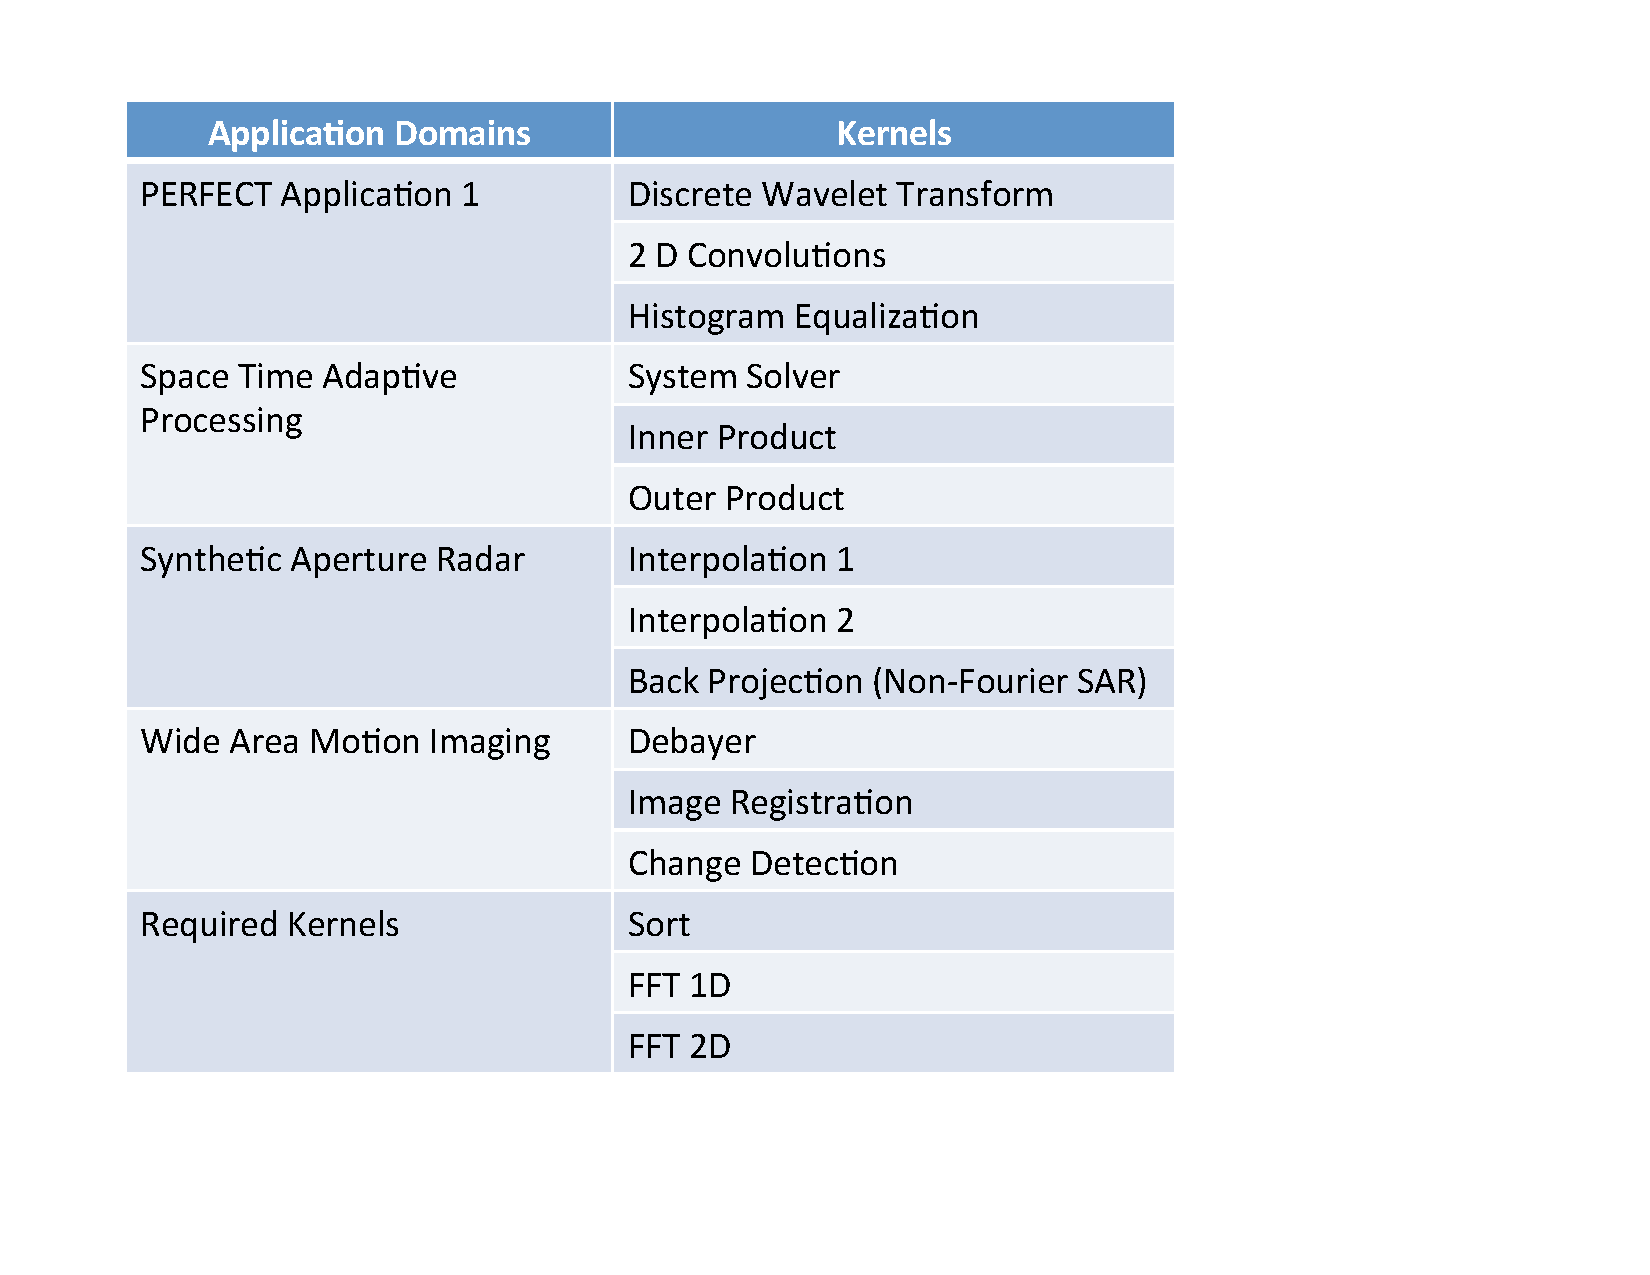
\includegraphics[width=1.0\textwidth]{figs/suite-taxonomy}
    \caption{Summary of the Perfect Benchmark Suite.}
    \label{fig:suite-taxonomy}
\end{figure}


%****************************************************************************
%****************************************************************************

\chapter{PERFECT Application 1 (PA1)}

%============================================================================
%============================================================================

\section{Kernel 1 -- 2D Convolution}
\label{sec:app1:2dconv}

\subsection{Motivation}

Convolution expresses the overlap of two functions $f$ and $g$ as $g$ is shifted
over $f$.  In image and signal processing, the function $f$ is the input image
or signal and $g$ is referred to as the filter.  The filter is shifted over and
applied to each pixel resulting in an output image of the same size.  Boundary
pixels must be handled carefully, usually by zero-padding the input.

The Gaussian filter is a filter whose impulse response is a Gaussian function.
When applied in two dimensions, each pixel in the output image represents a
weighted average of pixels in the neighborhood, where the weighting diminishes
in concentric circles around the focal point.  The Gaussian filter can be used
to reduce noise in images.

\subsection{Description}

The input image uses 32-bit unsigned pixels with a dynamic range of 16 bits per
pixel.
There are three sizes of input images: small (640x480), medium, (1920x1080),
and large (3840x2160).
The image width is $M$ pixels and the height is $N$ pixels.
The input image is convolved with a 9x9 Gaussian filter to produce
an output image with the same number of rows and columns.
The image is zero-padded so that the number of output pixels is equal to the
number of input pixels after convolution.
This process is repeated for each of 30 input frames.

The Gaussian 2D convolution is separable into two one-dimensional convolutions.
The one-dimensional filter is defined as $h[x]$.

\begin{equation}
h[x] =
 \begin{bmatrix}
  1 & 3 & 4 & 5 & 6 & 5 & 4 & 3 & 1
 \end{bmatrix}
\end{equation}

Multiplying by the transpose gives the complete 2D convolution filter $g[x,y]$.

\begin{equation}
  g[x,y] = h' \cdot h
\end{equation}

\begin{equation}
g[x,y] =
 \begin{bmatrix}
  1&   3&   4&   5&   6&   5&  4&    3&  1 \\
  3&   9&  12&  15&  18&  15&  12&   9&  3 \\
  4&  12&  16&  20&  24&  20&  16&  12&  4 \\
  5&  15&  20&  25&  30&  25&  20&  15&  5 \\
  6&  18&  24&  30&  36&  30&  24&  18&  6 \\
  5&  15&  20&  25&  30&  25&  20&  15&  5 \\
  4&  12&  16&  20&  24&  20&  16&  12&  4 \\
  3&   9&  12&  15&  18&  15&  12&   9&  3 \\
  1&   3&   4&   5&   6&   5&   4&   3&  1
 \end{bmatrix}
 \label{eq:gaussian}
\end{equation}

For the input image $f[x,y]$, the output of the benchmark is the convolution
$f[x,y] \ast g[x,y]$ with normalized pixel intensities.

\begin{equation}
 f[x,y] \ast g[x,y] = \frac{1}{1024} \sum_{n_1 = -4}^{4}
    \sum_{n_2 = -4}^{4} f[n_1,n_2] \cdot g[x-n_1,y-n_2]
\end{equation} 

\subsection{Specification}

\textbf{Input Data:}  30 frames; 16 bits per pixel; small (640x480), medium (1920x1080), large (3840x2160) \\ \\
\textbf{Output Data:}  30 frames, 16 bits per pixel,
with the 9x9 Gaussian
$g[x,y]$ in Eqn.~\ref{eq:gaussian} applied \\ \\
\textbf{Key Operations:}  Perform a 2D convolution of the image input with the 9x9 filter,
normalizing pixel intensities by $1/1024$

\subsection{Assessment}

\subsubsection{Correctness Assessment}

The 2D convolution kernel should be compared with the ``golden'' outputs provided.
Input and output image matrics can be visualized in MATLAB, Octave, or similar
environments.  Instructions can be found in \texttt{README.txt}.

\subsubsection{Performance Assessment}

The 2D convolution kernel nominally involves floating point arithmetic and
thus GFLOPS/W is one viable performance metric.
The unit of work for relative comparisons is the generation of a single
output pixel.
Each input data set includes $M \times N$ such units of work.

%============================================================================
%============================================================================

\section{Kernel 2 -- Discrete Wavelet Transform (DWT)}
\label{sec:app1:dwt}

\subsection{Motivation}

A wavelet is a single instance of a wave, isolated in time and frequency.
A wavelet transform represents a signal as a linear combination of wavelets.
The discrete wavelet transform is similar to the Fourier transform, except that
it captures both frequency and temporal information.  The discrete wavelet
transform can be used as a preconditioner to data compression in areas of
image and video processing.

The discrete wavelet transform to be implemented is the reversible 5/3 transform
used in the JPEG2000 specification for lossless compression~\cite{jpeg2000,Adams01wavelettransforms}.
When applied in two dimensions to an image, the discrete wavelet transform is
a combination of 1D transforms.  The DWT is applied first to each row, then to
each column.  This may be implemented using a transpose of rows to columns in
between each 1D transform.

\subsection{Description}

The input image uses 32-bit unsigned pixels with a dynamic range of 16 bits per
pixel.
There are three sizes of input images: small (640x480), medium, (1920x1080),
and large (3840x2160).
The image width is $M$ pixels and the height is $N$ pixels.
The 2D discrete wavelet transform is calculated by applying a 1D
DWT to the rows and then again to the columns.  This may be accomplished by
transposing the image between transforms.
This process is repeated for each of 30 input frames.

The reversible 5/3 transform takes an input $f[n]$ and produces a low-frequency
component $l[n]$ and a high frequency component $h[n]$.

\begin{equation}
 h[n] = f[2n+1] - \lfloor \frac{1}{2} (f[2n] + f[2n+2]) \rfloor
\end{equation}

\begin{equation}
 l[n] = f[2n] + \lfloor \frac{1}{4} (h[n] + h[n-1]) \rfloor
\end{equation}

The algorithm can be implemented in-place in the following manner.  At the end
of the computation, the low-frequency component is stored in the even locations
and the high-frequency component is stored in the odd locations.  Note that the
high frequency component must be calculated prior to the low frequency component
when computing in-place.

\begin{equation}
 f[2n+1] = f[2n+1] - \lfloor \frac{1}{2} (f[2n] + f[2n+2]) \rfloor
\end{equation}

\begin{equation}
 f[2n] = f[2n] + \lfloor \frac{1}{4} (f[2n-1] + f[2n+1]) \rfloor
\end{equation}

\subsection{Specification}

\textbf{Input Data:}  30 frames; 16 bits per pixel; small (640x480), medium (1920x1080), large (3840x2160) \\ \\
\textbf{Output Data:}   30 frames; 16 bits per pixel \\ \\
\textbf{Key Operations:}  Compute a 5/3 discrete wavelet transform of the input
  image

\subsection{Assessment}

\subsubsection{Correctness Assessment}

The discrete wavelet transform kernel should be compared with the ``golden'' outputs provided.
Input and output image matrics can be visualized in MATLAB, Octave, or similar
environments.  Instructions can be found in \texttt{README.txt}.

\subsubsection{Performance Assessment}

The unit of work for relative comparisons is the generation of a single
output pixel.
Each input data set includes $M \times N$ such units of work.

%============================================================================
%============================================================================

\section{Kernel 3 -- Histogram Equalization}
\label{sec:app1:histeq}

\subsection{Motivation}

The histogram of an image represents the probability distribution function of
the pixel values.  Histogram equalization increases the contrast of an image by
spreading the most frequent intensity values over a larger range.

\subsection{Description}

The input image uses 32-bit unsigned pixels with a dynamic range of 16 bits per
pixel.
There are three sizes of input images: small (640x480), medium, (1920x1080),
and large (3840x2160).

The first step computes a histogram of pixel values of the input
image.  The histogram places the value of each pixel $f[x,y]$ into one of $L$
uniformly-spaced buckets $h[i]$ (where $L = 2^{16}$).
The image width is $M$ pixels and the height is $N$ pixels.

\begin{equation}
 h[i] = \sum_{x=1}^{N} \sum_{y=1}^{M}
    \begin{cases}
    1, & \text{if $f[x,y]=i$}.\\
    0, & \text{otherwise}.
    \end{cases}
\end{equation}

Next, calculate the cumulative probability distribution function $cdf[j]$ on the
histogram $h[i]$.

\begin{equation}
 cdf[j] = \sum_{i = 1}^{j} h[i]
\end{equation}

Using the cumulative probability distribution function, scale each pixel in the
input image to produce an output image $g[x,y]$.
Output pixels are 32-bit unsigned integers and $L = 2^{16}$.
This process is repeated for each of 30 input frames.

\begin{equation}
 g[x,y] = \frac{cdf[ f[x,y] ] - cdf_{min}}{(N \cdot M) - cdf_{min}}
    \cdot (L - 1)
\end{equation}

$cdf_{min}$ is the smallest non-zero value of the cumulative probability
distribution function.

\subsection{Specification}

\textbf{Input Data:}  30 frames; 16 bits per pixel; small (640x480), medium (1920x1080), large (3840x2160) \\ \\
\textbf{Output Data:}  30 frames; 16 bits per pixel \\ \\
\textbf{Key Operations:}  Compute the histogram of input pixel values, compute
  the cumulative distribution of the histogram, and scale the input pixels to
  the output according to the cumulative distribution such that contrast is
  maximized.

\subsection{Assessment}

\subsubsection{Correctness Assessment}

The histogram equalization kernel should be compared with the ``golden'' outputs provided.
Input and output image matrics can be visualized in MATLAB, Octave, or similar
environments.  Instructions can be found in \texttt{README.txt}.

\subsubsection{Performance Assessment}

The histogram equalization kernel nominally involves floating point arithmetic and
thus GFLOPS/W is one viable performance metric.
The unit of work for relative comparisons is the generation of a single
output pixel.
Each input data set includes $M \times N$ such units of work.


%============================================================================
%============================================================================

\section{PA1 Application}
\label{sec:app1:app}


%****************************************************************************
%****************************************************************************

\chapter{Space-Time Adaptive Processing (STAP)}

Radar systems on an airborne platform must often mitigate the impact
of ground clutter (i.e., radar returns from the ground or structures), which can overwhelm other signals of interest.
Airborne movement further complicates the mitigation process because radar returns are spread in the Doppler dimension.
Space-time adaptive processing (STAP) algorithms address clutter by
adaptively computing and applying filters in both the spatial
(angular) and temporal (Doppler) domains.

The PERFECT Suite's STAP application domain is based upon the extended factored algorithm (EFA) introduced by DiPietro~\cite{DiPietro1992}.
The Suite's implementations are similar to RT\_STAP, a real-time STAP benchmark developed by the MITRE corporation~\cite{RT_STAP}.
In particular, the Suite uses the third-order Doppler-factored STAP benchmark case from RT\_STAP (i.e., the `hard' case).
An important difference between the Suite and RT\_STAP is that the Suite
excludes RT\_STAP's additional pre-processing.


%============================================================================
%============================================================================

\section{Motivation and Background}

Space-time adaptive processing largely utilizes standard linear algebra
functions, including inner and outer products and linear system
solves, as exemplified by the STAP kernel selection.
However, there are a few practical considerations that can substantially
impact performance.
For example, the inner and outer products operate on vectors
(space-Doppler snapshots) that are extracted from a larger data set
and thus memory access patterns are a key consideration for those
kernels.
In particular, explicitly forming a large set of contiguous
space-Doppler snapshot vectors and then calling inner or outer product functions
on that set of vectors may not be the best option.
Furthermore, the linear system solves are applied to a large set
of relatively small linear systems rather than to a small number
of large linear systems.
Finally, two of the three kernels operate on a three-dimensional
array and thus some memory reorganization (e.g., corner turns) may
be required to obtain high performance.

\subsection{Data Cube}
\label{sec:stap:datacube}

The input to STAP is a three-dimensional radar data cube consisting of
$L$ channels (or phase centers), $P$ pulses, and $N$ samples per pulse.
The $N$ samples per pulse are commonly termed range cells or range bins
because they sample at range (or time) intervals.
Because of the time scales involved, the range dimension is referred to
as fast-time and the pulse dimension is referred to as slow-time.
The $P$ pulses and $L$ channels add temporal and spatial diversity,
respectively, to the acquired data and thus those dimensions correspond
to space and time in space-time adaptive processing.
We represent the data cube as $\mathbf{x}$ and an individual entry with
channel $l$, range cell $n$, and pulse $p$ as $\mathbf{x}(l,n,p)$.
After the Doppler processing described in Section~\ref{sec:stap:doppler},
the data cube is represented by $\mathbf{X}$ and the entry corresponding
to channel $l$, range cell $n$, and Doppler bin $k$ is denoted
as $\mathbf{X}(l,n,k)$.

\subsection{Space-Doppler Snapshots}

The inner and outer product kernels are applied to space-Doppler
snapshot vectors extracted from the Doppler-processed data cube, $\mathbf{X}$.
A space-Doppler snapshot vector for range cell $n$ and Doppler bin $k$
includes all channels and the neighboring Doppler bins.
For the third-order Doppler-factored case, a neighborhood of three
Doppler bins is used and we denote this case by $T_{DOF}=3$ where
$T_{DOF}$ indicates the number of temporal degrees of freedom.
Using MATLAB-like notation, the snapshot column vector is
given by \texttt{vec($\mathbf{X}$(:,n,k-1:k+1))} where \texttt{vec} is
a function that vectorizes an array (i.e., it simply returns
\texttt{a(:)} for input array $\mathbf{a}$).
In cases where the Doppler indices would be out-of-bounds, they are
wrapped (i.e., $-1$ wraps to $K-1$ and $K$ wraps to 0, assuming
0-based indices).
The ordering of entries within the snapshot vector is arbitrary,
but must be consistent throughout the processing.
The snapshot operator is denoted as $\mathbf{S}(n,k)$ such that
$\mathbf{S}(n,k)$ can be interpreted as a column vector.

\subsection{Steering Vectors}

STAP will ultimately generate values for the range cell and Doppler
bin corresponding to each of $D$ specified steering vectors.
The definition of the steering vectors depend upon the geometry
of the antenna.
From the perspective of the STAP kernels and application, the steering
vectors are simply given as inputs and are thus not discussed further.
The $d$-th steering vector has dimension $(L \cdot T_{DOF}) \times 1$
and will be denoted by $\mathbf{v}(d)$.

\subsection{Doppler Processing (FFTs)}
\label{sec:stap:doppler}

The first stage of EFA converts from the pulse (time) domain to the
Doppler spectrum domain by applying a discrete Fourier transform (DFT) of
length $K$ to the $P$ pulses for each range cell and channel pair,
potentially after having applied a window function to the $P$ pulses.
Because the DFT will presumably be implemented via the FFT and the
FFT is already a kernel included with the PERFECT Suite, we do not
include a separate Doppler processing kernel for the STAP application.
However, for completeness we highlight that the incoming data cube
may not be stored in pulse-major order (in fact, that is unlikely
because pulse is the slowest temporal dimension), so either the
FFT would need to be applied in a strided fashion to non-contiguous
data or the data cube would need to be transformed into
pulse-major order.
This step is one of several involving radar data cubes where a
corner turn operation may be needed for efficiency.

\subsection{STAP}

The goal of STAP is ultimately to apply an
adaptive weighting vector, $\mathbf{w}$, to the snapshot
vectors in order to generate an output value for a specific
range cell, Doppler bin, and steering direction.
Therefore, a single complex output value $y$ will be given by
\begin{align}
    y = \mathbf{w}^{H} \mathbf{v}
\end{align}
where $\mathbf{v}$ is the steering direction and the superscript
$H$ denotes the Hermitian transpose operator.
The optimal weighting vector $\mathbf{w}_{opt}$ is given by
\begin{align}
    \mathbf{w}_{opt} = \gamma \mathbf{R}^{-1} \mathbf{v}
\end{align}
where $\mathbf{R}$ is the covariance matrix of the interference
(including clutter, noise, etc.) and $\gamma$ is a scalar
chosen to provide certain properties, such as
constant false alarm rate (CFAR) detection~\cite{MelvinSTAP}.

In practice, the exact covariance matrices are unknown
and must be estimated from the data.
Specifically, the covariance matrices are estimated by averaging
the outer products of a set of training space-Doppler snapshot
vectors.
Therefore, the covariance estimation comprises the outer product
STAP kernel.
After computing covariance estimates $\hat{\mathbf{R}}$, the
associated adaptive weighting vectors will be computed by solving
the linear systems given by $\hat{\mathbf{R}} \hat{\mathbf{w}} = \mathbf{v}$
using the linear system solver kernel.
Finally, the adaptive weighting vectors are applied to the snapshot
vectors and appropriately scaled during the adaptive weighting
kernel, which corresponds to the inner product computations.

\subsection{Parameter Sets}

The total workload and relative contribution of each kernel to the total
workload both depend upon the particular parameter set chosen for
the data cube and related processing.
The PERFECT suite includes small, medium, and large parameter values and
associated input and output data sets.
The parameters for the three cases are given in Table~\ref{tbl:stap:params}.

\begin{table}[t]
    \begin{center}
    \caption{STAP kernel parameters for the small, medium, and large test cases.}
    \begin{tabular}{|c|c|c|c|c|}
        \hline
        Parameter & Variable & Small & Medium & Large \\ \hline
        Spatial channels/elements & $L$ & 4 & 6 & 8 \\ \hline
        Pulses per CPI & $P$ & 128 & 128 & 128 \\ \hline
        Doppler bins & $K$ & 256 & 256 & 256\\ \hline
        Range bins & $N$ & 512 & 1024 & 4096 \\ \hline
        Range bins per training block & $N_R$ & 32 & 64 & 64 \\ \hline
        Temporal degrees of freedom & $T_{DOF}$ & 3 & 3 & 3 \\ \hline
        Steering vectors & $D$ & 16 & 16 & 16 \\ \hline
    \end{tabular}
    \label{tbl:stap:params}
    \end{center}
\end{table}

%============================================================================
%============================================================================

\section{STAP Kernel 1 -- Outer Product: \\ Covariance Estimation}
\label{sec:stap:cov}

\subsection{Description}

STAP requires an estimate of the covariance for a given range cell
and Doppler bin in order to calculate the associated adaptive weights.
One option for making such an estimate is to train based on the
acquired data itself.
The RT\_STAP benchmark employs a block training strategy that
corresponds to the covariance estimation kernel.
In particular, the range dimension is blocked into $M$ disjoint blocks
with $N_R$ contiguous range cells such that $M = N / N_R$.
For simplicity, we assume that $N_R$ evenly divides $N$.

The covariance estimate for range block $b$ and Doppler bin $k$ is then
\begin{align}
\hat{\mathbf{R}}(b,k) = \frac{1}{N_R} \sum_{r=b \cdot N_R}^{(b+1)\cdot N_R-1} {\mathbf{S}(r,k) \mathbf{S}^H(r,k)}.
\end{align}
Thus, the covariance estimation kernel generates $M \times K$
covariance matrices.
Note that many training strategies are available.
For example, a sliding window could be utilized such that
a unique covariance matrix is generated for each range cell $n$.
However, the sliding window strategy would generate
$N \times K$ covariance matrices, which would correspondingly
increase the computational load for the linear system solver
by a factor of $N_R$.
Therefore, the block training strategy is in part an optimization
to reduce the computational burden of solving for the adaptive weights.
While this benchmark does not focus on training strategies, the
RMB rule, named after the authors who observed it, indicates that
approximately $2 N_R L$ training samples corresponds to a roughly
3 dB performance loss under certain statistical assumptions~\cite{Reed1974}.

\subsection{Specification}
\label{sec:stap:cov_generation:spec}

\textbf{Input Data:} A {3D} complex data cube of dimension $N \times K \times L$. \\ \\
\textbf{Output Data:} $(N/N_R) \times K$ complex matrices, each of dimension
$(L \cdot T_{DOF}) \times (L \cdot T_{DOF})$. \\ \\
\textbf{Key Operations:} Each output matrix is the mean of $N_R$ outer products
of $(L \cdot T_{DOF})$-length vectors.  The output matrices are conjugate
symmetric, so symmetry can be exploited to reduce computation and/or storage.

\subsection{Assessment}

\subsubsection{Correctness Assessment}

The outer product kernel can be assessed using the SNR metric described
in Section~\ref{sec:correctness:snr}.
For the reference implementation, a single SNR value is computed over all
covariance matrices (i.e., over all of the produced output).
Although no specific correctness threshold is yet defined, SNR values in the
range of $100$ dB are reasonable.

\subsubsection{Performance Assessment}

The outer product kernel nominally involves floating point arithmetic and thus
GFLOPS/W is one viable performance metric.
The unit of work for relative comparisons is the generation of a single complex
covariance matrix of size $(L \cdot T_{DOF}) \times (L \cdot T_{DOF})$, although
symmetry may be exploited for more compact storage.
Each input data set includes $(N/N_R) \times K$ such units of work.

%============================================================================
%============================================================================

\section{STAP Kernel 2 -- Linear System Solver:\\ Weight Generation}

\subsection{Description}

The covariance matrices $\hat{\mathbf{R}}(b,k)$ generated by the
kernel described in Section~\ref{sec:stap:cov} are conjugate symmetric
and positive semi-definite.
Furthermore, due to receiver noise, the covariance matrices are
typically positive definite with a suitable amount of
training~\cite[Chapter~10]{POMRv2}.
For the purposes of the PERFECT Suite, the covariance matrices
can be assumed to be positive definite and conjugate symmetric.

While the RT\_STAP benchmark utilizes QR decomposition, any
suitable method for solving the linear systems given by
\begin{align}
    \hat{\mathbf{R}}(b,k) \hat{\mathbf{w}}(b,k,d) = \mathbf{v}(d)
\end{align}
is sufficient.
The explicit inverses, $\hat{\mathbf{R}}^{-1}(b,k)$, are not needed
and the systems have $D$ associated right-hand sides corresponding
to the $D$ steering directions.
Furthermore, an additional weighting scalar $\hat{\gamma}$ can be
included to provide desired qualities.
In this case, the scalar is given as
\begin{align}
    \hat{\gamma} & = (\hat{\mathbf{w}}^H \mathbf{v})^{-1}
        = ((\hat{\mathbf{R}}^{-1} \mathbf{v})^H \mathbf{v})^{-1}
        = (\mathbf{v}^H \hat{\mathbf{R}}^{-H} \mathbf{v})^{-1}
\end{align}
where we have dropped the indices for clarity.
$\hat{\mathbf{R}}$ is Hermitian positive definite, so the Hermitian of
its inverse, $\hat{\mathbf{R}}^{-H}$, is also positive definite.
Therefore, $\mathbf{v}^H \hat{\mathbf{R}}^{-H} \mathbf{v}$ is
a real scalar and its inverse is simply $1/(\mathbf{v}^H \hat{\mathbf{R}}^{-H} \mathbf{v})$.
With this definition for $\hat{\gamma}$, the weighted results are normalized
such that $\hat{\gamma} \hat{\mathbf{w}}^H \mathbf{v} = 1$.
Because the weighting scalars are computed from $\hat{\mathbf{w}}$ and
$\mathbf{v}$, they can either be computed and stored explicitly or
computed on-the-fly as part of the adaptive weighting described
in Section~\ref{sec:stap:adaptive_weighting}.

\subsection{Specification}
\label{sec:stap:weight_generation:spec}

\textbf{Input Data:} $(N/N_R) \times K$ complex matrices, each of dimension
$(L \cdot T_{DOF}) \times (L \cdot T_{DOF})$, and $D$ complex steering vectors
of length $L \cdot T_{DOF}$. \\ \\
\textbf{Output Data:} $(N/N_R) \times K \times D$ complex weighting vectors,
each of length $L \cdot T_{DOF}$. \\ \\
\textbf{Key Operations:}
Solve  $(N/N_R) \times K \times D$ linear systems $\mathbf{Ax = b}$ where
matrix $\mathbf{A}$ is $(L \cdot T_{DOF}) \times (L \cdot T_{DOF})$ and $\mathbf{x}$
and $\mathbf{b}$ are both $(L \cdot T_{DOF})$-length column vectors.
The matrices can be assumed to be Hermitian positive definite.
A single matrix $\mathbf{A}$ will be reused with $D$ right-hand sides.

\subsection{Assessment}

\subsubsection{Correctness Assessment}

The system solver kernel can be assessed using the SNR metric described
in Section~\ref{sec:correctness:snr}.
For the reference implementation, a single SNR value is computed over all
weighting vectors (i.e., over all of the produced output).
Although no specific correctness threshold is yet defined, SNR values in the
range of $100$ dB are reasonable.

\subsubsection{Performance Assessment}

The system solver kernel nominally involves floating point arithmetic and
thus GFLOPS/W is one viable performance metric.
The unit of work for relative comparisons is the generation of $D$ complex
steering vectors of length $L \cdot T_{DOF}$.
Each input data set includes $(N/N_R) \times K$ such units of work.

%============================================================================
%============================================================================

\section{STAP Kernel 3 -- Inner Product: \\ Adaptive Weighting}
\label{sec:stap:adaptive_weighting}

\subsection{Description}

Finally, the adaptive weights are applied to the snapshot vectors
to form the final STAP output.
This step corresponds to a complex inner product and is given by
\begin{align}
    \mathbf{y}(n,k,d) = \hat{\gamma}(b,k,d) \hat{\mathbf{w}}^H(b,k,d) \mathbf{S}(n,k)
    \label{eq:stap:gamma}
\end{align}
for range cell $n$, Doppler bin $k$, steering direction $d$, and
range block $b$ corresponding to range cell $n$.
The same weighting vector and associated scalar is used for all
range cells within a range block and thus the block training
strategy also potentially reduces memory traffic during the adaptive
weighting, although it does not necessarily impact the
number of floating point operations.

\subsection{Specification}
\label{sec:stap:adaptive_weighting:spec}

\textbf{Input Data:}
A {3D} complex data cube of dimension
$N \times K \times L$ and $(N/N_R) \times K \times D$ complex
weighting vectors, each of length $L \cdot T_{DOF}$. \\ \\
\textbf{Output Data:}
A {3D} complex data cube of dimension $N \times K \times D$. \\ \\
\textbf{Key Operations:}
Compute $N \times K \times D$ complex inner products over $L \cdot T_{DOF}$-length
vectors.  Furthermore, an additional $K \times (N/N_R) \times D$ complex
inner products over vectors of length $L \cdot T_{DOF}$ will be required for
the scaling given by $\hat{\gamma}$ in Eq.~(\ref{eq:stap:gamma}).

\subsection{Assessment}

\subsubsection{Correctness Assessment}

The inner product kernel can be assessed using the SNR metric described
in Section~\ref{sec:correctness:snr}.
For the reference implementation, a single SNR value is computed over all
weighting vectors (i.e., over all of the produced output).
Although no specific correctness threshold is yet defined, SNR values in the
range of $100$ dB are reasonable.

\subsubsection{Performance Assessment}

The inner product kernel nominally involves floating point arithmetic and
thus GFLOPS/W is one viable performance metric.
The unit of work for relative comparisons is the generation of a single
complex output sample.
Each input data set includes $N \times K \times D$ such units of work.


%============================================================================
%============================================================================

\section{STAP Application}
\label{sec:stap:app}

The kernels and operations described above can be merged into a full
space-time adaptive processing pipeline, or STAP application.

\subsection{Description}

In addition to the three PERFECT suite STAP kernels, the STAP application
adds the Doppler processing step described in Section~\ref{sec:stap:doppler}.
The application arranges the operations in the following order, with the
outputs from one stage forming the input to the next:

\begin{enumerate}
    \item Doppler processing -- Corner turns, windowing, and FFTs
    \item Kernel 1 -- Outer products -- Covariance estimation
    \item Kernel 2 -- Linear system solves -- Weight generation
    \item Kernel 3 -- Inner product -- Adaptive weighting
\end{enumerate}

The corner turns included in the Doppler processing stage convert the data
to pulse-major order to apply FFTs to contiguous array and then re-convert
the data to range-major order prior to kernel 1 so that the kernel 1
implementation remains the same for the kernel benchmark and application.
However, the corner turns are applied only for convenience and an optimized
implementation could arrange the data cube differently and modify the
kernel implementations accordingly.

\subsection{Specification}

\textbf{Input Data:} A {3D} complex data cube of dimension $N \times P \times L$. \\ \\
\textbf{Output Data:}
A {3D} complex data cube of dimension $N \times K \times D$. \\ \\
\textbf{Key Operations:} 
The Doppler processing stage involves corner turns, windowing (i.e., element-wise
multiplications), and FFTs.
The three kernels following Doppler processing involve the same operations
as described in Sections~\ref{sec:stap:cov_generation:spec}, \ref{sec:stap:weight_generation:spec},
and \ref{sec:stap:adaptive_weighting:spec}.

\subsection{Assessment}

\subsubsection{Correctness Assessment}

The full application can be assessed using the SNR metric described
in Section~\ref{sec:correctness:snr}.
For the reference implementation, a single SNR value is computed over all
output values.
The SNR threshold for the full application could resaonably be lower than
for individual kernels due to the cumulative loss of precision from one
kernel to the next.
For the reference implementation, the SNR relative to a fully double precision
implementation is $80$ dB, which is reasonable relative to a threshold
of $100$ dB for the individual kernels.

\subsubsection{Performance Assessment}

The STAP application nominally involves floating point arithmetic and thus
GFLOPS/W is one viable performance metric.
The unit of work for relative comparisons is the generation of a single
complex output sample.
Each input data set includes $N \times K \times D$ such units of work.
Note, however, that workload scales with other parameters, such as
$T_{DOF}$.
Therefore, the units of work are only comparable between similarly
parameterized variants of STAP.

%****************************************************************************
%****************************************************************************

\chapter{Synthetic Aperture Radar (SAR)}

%============================================================================
%============================================================================

\section{Motivation and Background}

Synthetic aperture radar (SAR) is a radar-based imaging modality capable
of producing high-resolution imagery from an airborne platform.
Rather than utilizing a large aperture to achieve high resolution, SAR
synthesizes a large aperture using platform motion and then forms an
image using data corresponding to the pulses acquired over the synthetic
aperture.
The amount of data needed for image formation is a function of the radar
system parameters, desired image resolution, and coverage area.

The SAR kernels correspond to two alternative methods of image formation.
In particular, the two interpolation kernels relate to the polar format
algorithm (PFA), which is a Fourier-based approach, and the backprojection
kernel represents the inner loop for the backprojection algorithm.
Backprojection has a higher computational complexity than PFA, but PFA has
some restrictions in terms of imaging geometry compared to the more general
backprojection algorithm.
For example, PFA assumes that the spherical wavefronts incident upon a
scene are planar and the extent to which that assumption holds depends
upon the specifics of the collection scenario.

\subsection{SAR Data}

Although SAR can utilize a three-dimensional radar data cube similar to
that presented for STAP in Section~\ref{sec:stap:datacube}, we consider
only the two-dimensional case of $P$ radar pulses and $N$ 
complex-valued samples per pulse.
In the case of backprojection, the $N$ samples per pulse will be upsampled
to $N_{BP}$ samples per pulse prior to the backprojection kernel.
The output of SAR processing will be a complex-valued image of dimension
$N_x \times N_y$, although in the case of PFA an additional 2D IFFT would
need to be performed after the interpolations in order to produce an
output image.
The backprojection kernel, on the other hand, will directly produce an
output image.

\subsection{Polar Format Algorithm (PFA)}

Data collected during a SAR acquisition corresponds to the Fourier
transform of scene reflectivity and thus an image can be reconstructed
via inverse Fourier transforms.
However, the sampled data points correspond to a polar grid in Fourier
space and thus the fast Fourier transform (FFT), which operates on a rectangular
grid, cannot be used directly.
In order to leverage the FFT, the data is first interpolated onto a
rectangular grid.
While the required interpolation is notionally two-dimensional, it is
typical to assume separability and perform the interpolation as two
one-dimensional interpolation steps.
The two PERFECT suite SAR interpolation kernels correspond to these one-dimensional
interpolations that achieve the polar to rectangular coordinate conversion.
Both PFA interpolation kernels utilize a truncated sinc interpolation footprint
of width $T_{PFA}$.
If we assume that the number of pulses, samples per pulse, and pixels-per-side
of the formed image are all approximately $N$, then the computational complexity
of PFA is given by $\mathcal{O}(N^2 \log N)$.

\subsection{Backprojection (BP)}

The backprojection, or backpropagation, algorithm is a method of image
formation that directly integrates a contribution from each pulse into
each pixel.
Thus, the computational complexity for BP is $\mathcal{O}(P\cdot N_x\cdot N_y)$.
For the nominal case where the number of pulses and pixels-per-side of the
formed image are comparable (e.g., $N$), the computational complexity of
backprojection is $\mathcal{O}(N^3)$.

Although it is not included as a separate kernel, it is common to upsample
data in the range dimension prior to backprojection in order to effectively
improve the interpolation quality (i.e., high order interpolation during
upsampling followed by lower-order interpolation during backprojection).
The upsampling can be performed via an FFT with zero-padding in the Fourier
domain and is thus already covered by the 1D FFT in the required kernel
section.
The backprojection kernel operates on data that has already been upsampled
and thus the samples-per-pulse value will be $N_{BP} \ge N$.

\subsection{Parameter Sets}

The total workload of each kernel depends upon the particular parameter
set chosen for the input data set and related processing.
The PERFECT suite includes small, medium, and large parameter values and
associated input and output data sets.
The parameters for the three cases are given in Table~\ref{tbl:sar:params}.

\begin{table}[t]
    \begin{center}
    \caption{SAR kernel parameters.}
    \begin{tabular}{|c|c|c|c|c|}
        \hline
        Parameter & Variable & Small & Medium & Large \\ \hline
        Pulses & $P$ & 512 & 1024 & 2048 \\ \hline
        Range bins & $N$ & 512 & 1024 & 2048 \\ \hline
        Upsampled range bins (BP) & $N_{BP}$ & 4096 & 8192 & 16384 \\ \hline
        Resampled range bins (PFA) & $N_{PFA}$ & 512 & 1024 & 2048 \\ \hline
        Resampled pulses (PFA) & $P_{PFA}$ & 512 & 1024 & 2048 \\ \hline
        Image size & $N_x \times N_y$ & $512 \times 512$ & $1024 \times 1024$ & $2048 \times 2048$ \\ \hline
        Carrier frequency & $f_c$ & 10~GHz & 10~GHz & 10~GHz \\ \hline
        PFA interpolation width & $T_{PFA}$ & 13 & 13 & 13 \\ \hline
    \end{tabular}
    \label{tbl:sar:params}
    \end{center}
\end{table}


%============================================================================
%============================================================================

\section{SAR Kernel 1 -- Interpolation 1: \\ PFA Range Interpolation}

\subsection{Description}

Both PFA kernels utilize the normalized sinc function given by
\begin{align*}
\operatorname{sinc}(x) = \frac{\sin(\pi x)}{\pi x}
\end{align*}
to interpolate from a given input coordinate grid to a given output 
coordinate grid.
The first interpolation is applied along the range dimension and
the second is applied along the azimuth (pulse) dimension.
Furthermore, the interpolation kernel is weighted by a real-valued window
function $\mathbf{w}$.
The interpolation for both SAR kernels takes the following form~\cite[Chapter~6]{POMRv2}:
\begin{align}
    \mathbf{g}(m) = \frac{\Delta y}{\Delta x} \sum_{k=-(T_{PFA}-1)/2}^{(T_{PFA}-1)/2} \mathbf{f}(k+n(\mathbf{y_m}))
        \mathbf{w}(k) \operatorname{sinc}\left(\frac{\mathbf{y}_m - \mathbf{x}_{k+n(\mathbf{y}_m)}}{\Delta x}\right)
    \label{eq:sar:tsinc_interp}
\end{align}
where $\mathbf{f}$ and $\mathbf{g}$ are the input and output functions,
$\mathbf{x}$ and $\mathbf{y}$ are the input and output coordinates,
$\Delta x$ and $\Delta y$ are the average spacing for the input and output coordinates,
$\mathbf{w}$ is the window function defined over the interpolation kernel, and
$n(\mathbf{y}_m)$ is the index of the coordinate in $\mathbf{x}$ nearest to $\mathbf{y}_m$.
In other words, we resample the function $\mathbf{f}$ defined at coordinates
$\mathbf{x}$ to the function $\mathbf{g}$ defined at coordinates $\mathbf{y}$.
In the case where the interpolation kernel extends outside the domain of $\mathbf{f}$
(e.g., when $k+n(\mathbf{y_m}) < 0$), values of zero replace $\mathbf{f}$.

For PFA range interpolation, Eq.~(\ref{eq:sar:tsinc_interp}) is applied along
the range (fast-time) dimension.
The input sample coordinates vary with pulse, but they are uniformly spaced
for a given pulse.
Furthermore, it can be assumed that the input coordinates are
monotonically increasing.
The equidistant input sampling can be exploited during interpolation 
when computing the nearest input neighbor index $n(\mathbf{y}_m)$ to
output coordinate $\mathbf{y}_m$.
The reference implementation exploits the uniform sample spacing of the
input coordinates to compute $n()$ via a closed form expression.

\subsection{Specification}

\textbf{Input Data:} A {2D} $P \times N$ complex data matrix,
a {2D} $P \times N$ array of input coordinates, a {1D} array
of $N_{PFA}$ output coordinates, and a PFA interpolation width ($T_{PFA}$). \\ \\
\textbf{Output Data:} 
A resampled {2D} $P \times N_{PFA}$ complex data matrix. \\ \\
\textbf{Key Operations:} For each complex output sample, compute the nearest neighbor among
the input coordinates and apply a $T_{PFA}$-width truncated sinc interpolation kernel
to the associated complex input data values.
The input coordinates can be assumed to be both monotonically increasing and uniformly
spaced for a given pulse, but may vary from pulse to pulse.

\subsection{Assessment}

\subsubsection{Correctness Assessment}

The PFA range interpolation kernel can be assessed using the SNR metric described
in Section~\ref{sec:correctness:snr}.
For the reference implementation, a single SNR value is computed over all
samples (i.e., over all of the produced output).
Although no specific correctness threshold is defined, SNR values in the
range of $100$ dB are reasonable.

\subsubsection{Performance Assessment}

The PFA range interpolation kernel nominally involves floating point arithmetic
and thus GFLOPS/W is one viable performance metric.
The unit of work for relative comparisons is the generation of a single complex
output sample.
Each input data set includes $P \times N_{PFA}$ such units of work.

%============================================================================
%============================================================================

\section{SAR Kernel 2 -- Interpolation 2: \\ PFA Azimuth Interpolation}

\subsection{Description}

PFA azimuth interpolation is similar to range interpolation and still utilizes
Eq.~(\ref{eq:sar:tsinc_interp}) for the interpolation model.
The azimuth interpolation is applied to the output of the range interpolation
kernel and resamples the data along the azimuth (pulse) dimension.
However, for azimuth interpolation, it is no longer the case that
the input spacing is generally uniform for a given range frequency.%
\footnote{The initial input data set does have uniform sample spacing
along the input azimuth coordinates, but that is due to having used an
idealized simulation to generate the data. Platform velocity or trajectory
variation during an acquisition would generate non uniformly spaced
azimuth samples.}
Therefore, the computation of the nearest input neighbor index for a given
output coordinate may be more general for azimuth interpolation than
range interpolation.
The reference implementation employs a binary search method to compute
$n()$ for the azimuth case, but any method of computing $n()$ over a
non-uniform input sample grid is acceptable.
It can be assumed that the input coordinates are monotonically increasing.

\subsection{Specification}

\textbf{Input Data:} A {2D} $P \times N_{PFA}$ complex data matrix,
a {2D} $P \times N_{PFA}$ array of input coordinates, a {1D} array
of $P_{PFA}$ output coordinates, and a PFA interpolation width ($T_{PFA}$). \\ \\
\textbf{Output Data:} 
A resampled {2D} $P_{PFA} \times N_{PFA}$ complex data matrix. \\ \\
\textbf{Key Operations:} For each complex output sample, compute the nearest neighbor among
the input coordinates and apply a $T_{PFA}$-width truncated sinc interpolation kernel
to the complex input data values.
The input coordinates can be assumed to be monotonically increasing, but not necessarily
uniformly spaced, for a given range frequency.
Furthermore, the input coordinates may vary from range frequency to range frequency.

\subsection{Assessment}

\subsubsection{Correctness Assessment}

The PFA azimuth interpolation kernel can be assessed using the SNR metric described
in Section~\ref{sec:correctness:snr}.
For the reference implementation, a single SNR value is computed over all
samples (i.e., over all of the produced output).
Although no specific correctness threshold is defined, SNR values in the
range of $100$ dB are reasonable.

Furthermore, the output of the PFA azimuth interpolation can be visualized
as an image after applying a {2D} inverse FFT.
The TAV suite includes the script \texttt{generate\_pfa\_image.m} for
applying the 2D IFFT and displaying the resulting image.
This script can be run in MATLAB, Octave, or other similar environments.
Sample output from the reference kernel implementation is shown in
Figure~\ref{fig:pfa_output}.
This data set included three simulated point reflectors that manifest
as two-dimensional sinc functions in the output image.

\begin{figure}
    \centering
    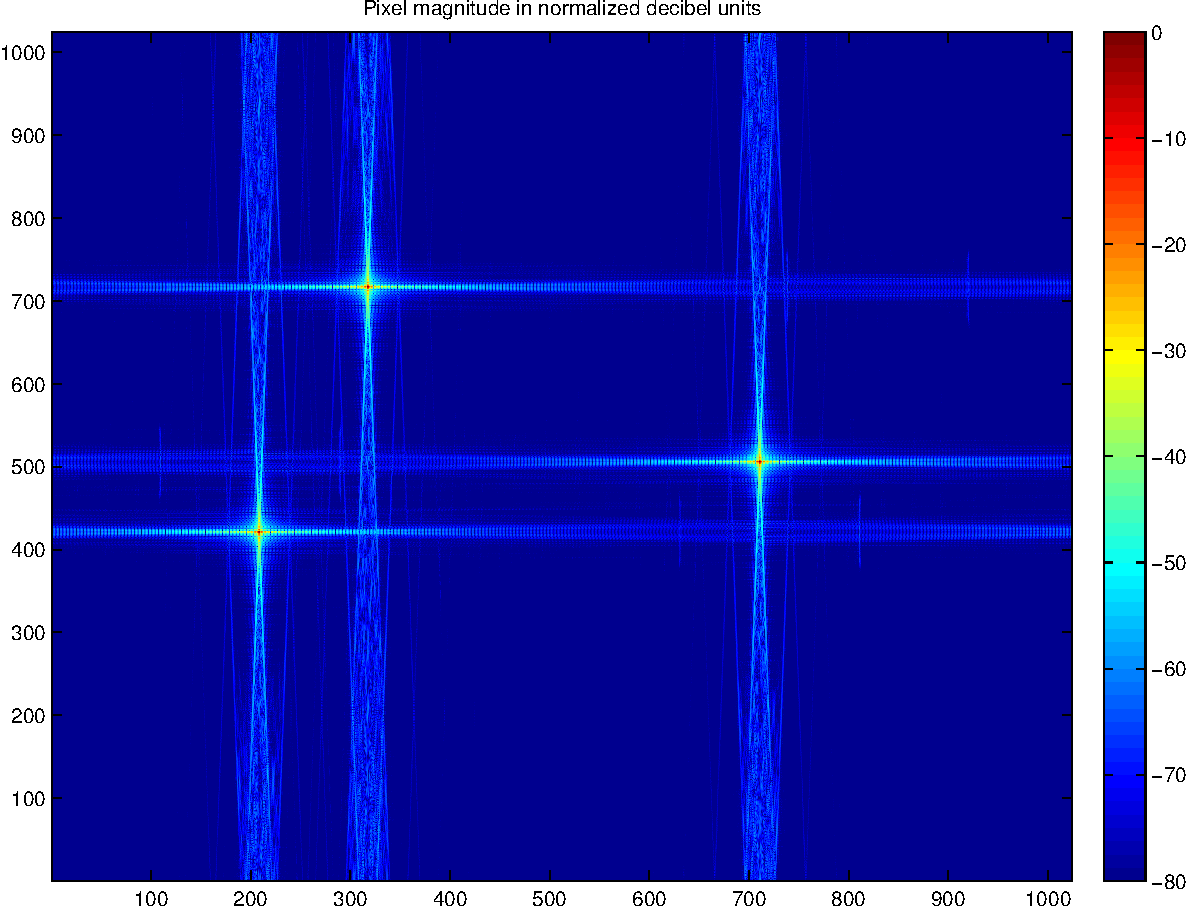
\includegraphics[width=0.75\textwidth]{figs/sample_pfa_output}
    \caption{Sample output image generated by applying a 2D inverse FFT to
the PFA kernel 2 (azimuth interpolation) output.  %
Pixel values correspond to normalized magnitude in decibel scale.}
    \label{fig:pfa_output}
\end{figure}

\subsubsection{Performance Assessment}

The PFA azimuth interpolation kernel nominally involves floating point arithmetic
and thus GFLOPS/W is one viable performance metric.
The unit of work for relative comparisons is the generation of a single complex
output sample.
Each input data set includes $P_{PFA} \times N_{PFA}$ such units of work.

%============================================================================
%============================================================================

\section{SAR Kernel 3 -- Backprojection}

\subsection{Description}

The backprojection algorithm is described in many papers and
textbooks~\cite{GorhamSPIE2010,MunsonIEEE1983,DesaiTIP1992},
often in the context of similar image formation algorithms from medical
imaging via x-ray computed tomography.
Backprojection takes as input the location of the imaging platform for
each pulse, the location of each output pixel, and the $P \times N_{BP}$
data set.
For pixel $k$ and pulse $p$, backprojection consists of the following
steps:
\begin{itemize}
    \item Compute the distance from the platform to the pixel
    \item Convert the distance to an associated position (range) in the data set
    \item Sample at the computed range via linear interpolation
    \item Scale the sampled value by a matched filter to form the pixel contribution
    \item Accumulate the contribution into the pixel.
\end{itemize}

Given input data $\mathbf{x}$ of dimension $P \times N_{BP}$, per-pulse platform
positions $\mathbf{v}$, and output image $\mathbf{y}$, the $k$th output pixel
with location $\mathbf{a}_k = (x_k,y_k,z_k)$ is given by
\begin{align}
    \mathbf{y}_k = \sum_{p=1}^{P} \tilde{\mathbf{x}}(p, r(p,k)) \cdot e^{j \cdot 2 \cdot k_u \cdot r(p,k)}
    \label{eq:sar:bp}
\end{align}
where $r(p,k)=||\mathbf{a}_k-\mathbf{v}_p||$ is the distance from the platform location at pulse $p$ to
pixel $k$ and the tilde on $\mathbf{x}$ indicates linear interpolation in
range to estimate the value at position $r(p,k)$.
The value $k_u$ is equal to $2\pi f_c /c$ where $f_c$ is the carrier frequency
of the radar waveform and $c$ is the speed of light.
The complex exponential $e^{j \theta}$ is equivalent to $\cos(\theta) + j \sin(\theta)$
via Euler's formula and thus a sine and cosine computation is implied
in Equation~(\ref{eq:sar:bp}) for each pixel-pulse pair.
While $k_u$ is a constant from the perspective of an implementation, its
value will impact the magnitude of the argument for the sine and cosine
calculations and thus may have a direct impact on performance due to
argument reduction.

The backprojection algorithm is shown in pseudocode form in Algorithm~\ref{alg:sar:bp}
where the linear interpolation mechanics are made explicit.
The values $R_0$ and $\Delta R$ in Algorithm~\ref{alg:sar:bp} denote
the distance to the first range bin and the distance per range bin, respectively.
$R_0$ and $\Delta R$ are constants from the perspective of the implementation and are
used to convert the computed distance (range) into an array index for linear
interpolation.

\begin{algorithm}
    \begin{algorithmic}[1]
        \FORALL{pixels $k$}
            \STATE{$\mathbf{y}_k = 0$}
            \FORALL{pulses $p$}
                \STATE{$R = || \mathbf{a}_k - \mathbf{v}_p || $} \COMMENT{Distance from platform to voxel}
                \STATE{$\text{bin} = \lfloor (R-R_0)/\Delta R \rfloor$} \COMMENT{Range bin (integer)}
                \IF{$\text{bin} \in [0, N_{BP}-2]$}
                    \STATE{$w = (R-R_0)/\Delta R - \text{bin}$}
                    \\ \COMMENT{Data sampled using linear interpolation}
                    \STATE{$s = (1-w)\cdot \mathbf{x}(p,\text{bin}) + w\cdot \mathbf{x}(p,\text{bin}+1)$}
                    \STATE{$\mathbf{y}_k = \mathbf{y}_k + s \cdot e^{j \cdot k_u \cdot R}$}
                \ENDIF
            \ENDFOR
        \ENDFOR
    \end{algorithmic}
    \caption{Backprojection pseudocode.}
    \label{alg:sar:bp}
\end{algorithm}

\subsection{Specification}

\textbf{Input Data:} A {2D} $P \times N_{BP}$ complex data matrix, a 
vector of $P$ three-dimensional platform positions, and output pixel coordinates.
While backprojection can generate pixel data for arbitrary coordinates (given proper
data support), the output image is centered at the origin and is assumed rectangular
with uniform pixel spacing.
The output image is parameterized by the pixel spacing $\Delta x$ and
$\Delta y$ for the $x$ and $y$ dimensions, respectively. \\ \\
\textbf{Output Data:} 
A complex image of dimension $N_x \times N_y$. \\ \\
\textbf{Key Operations:} For each pixel and pulse, there is a distance calculation
(including a square root), a linear interpolation, a complex exponential computation,
and a complex multiplication and accumulation.

\subsection{Assessment}

\subsubsection{Correctness Assessment}

The backprojection kernel can be assessed using the SNR metric described
in Section~\ref{sec:correctness:snr}.
For the reference implementation, a single SNR value is computed over all
pixels (i.e., over all of the produced output).
Although no specific correctness threshold is defined, SNR values in the
range of $100$ dB are reasonable.

Furthermore, the backprojection kernel generates an output image and that
image can be visualized and compared against the ``golden'' output image.
The TAV suite includes the script \texttt{display\_bp\_image.m} 
for displaying the generated images.
This script can be run in MATLAB, Octave, or other similar environments.
Sample output from the reference kernel implementation is shown in
Figure~\ref{fig:bp_output}.
Note that the output images generated by PFA and BP differ in several
respects and thus should not be compared against one another for
validation purposes.

\begin{figure}
    \centering
    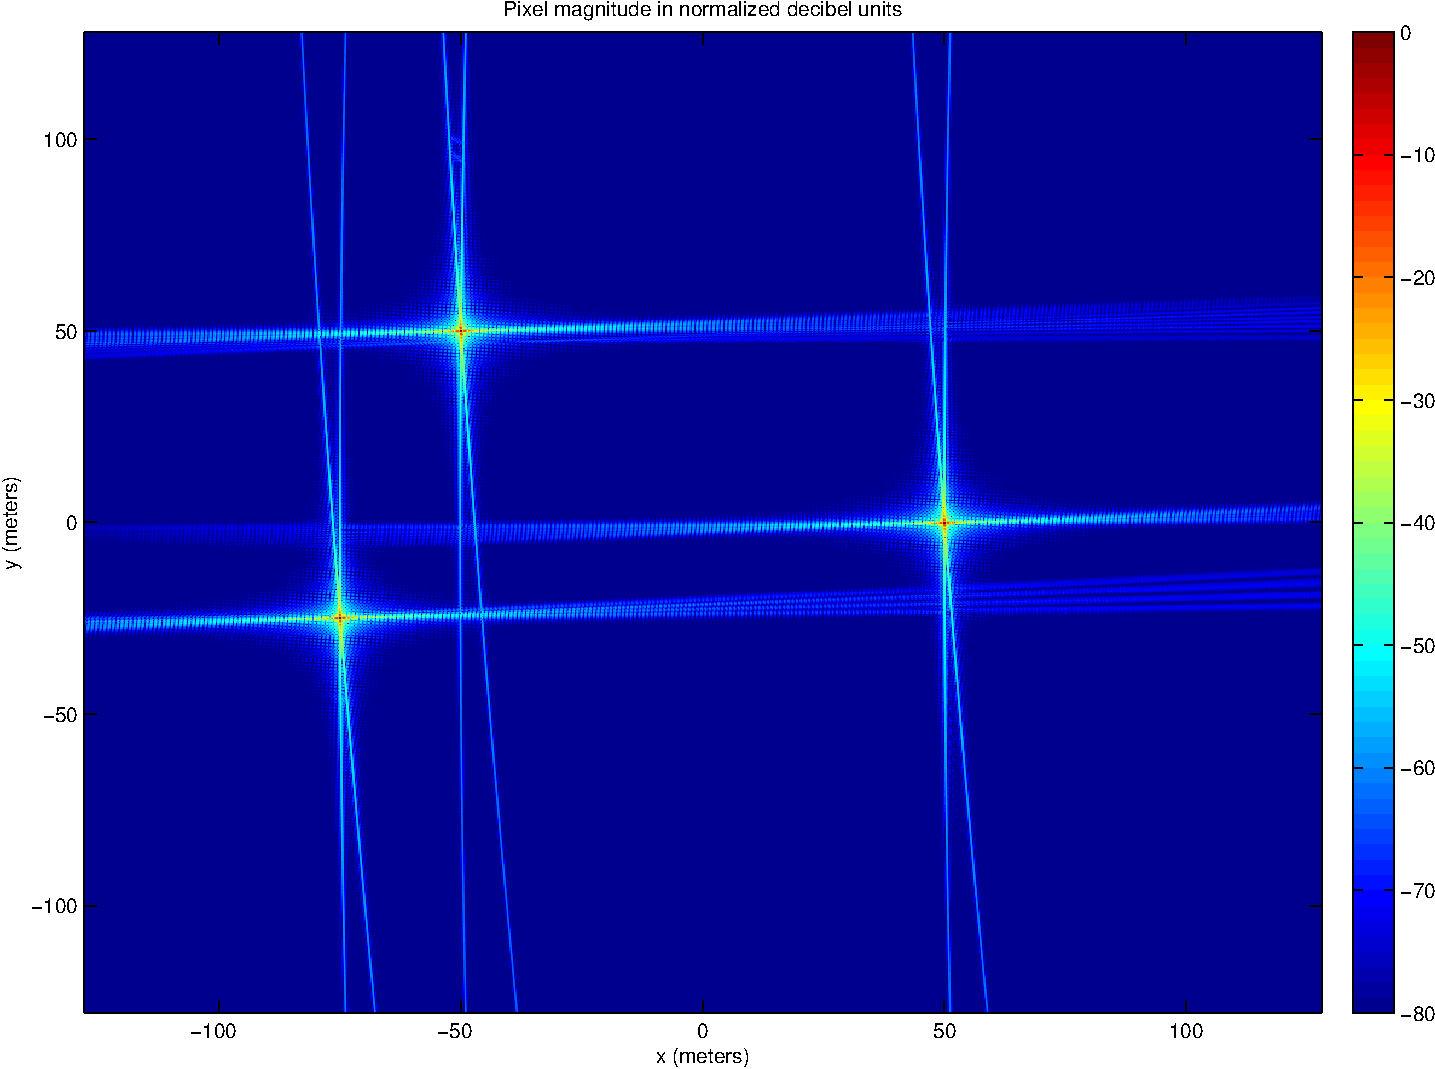
\includegraphics[width=0.75\textwidth]{figs/sample_bp_output}
    \caption{Sample output image generated by the SAR backprojection kernel.  %
Pixel values correspond to normalized magnitude in decibel scale.}
    \label{fig:bp_output}
\end{figure}

\subsubsection{Performance Assessment}

The backprojection kernel nominally involves floating point arithmetic
and thus GFLOPS/W is one viable performance metric.
The unit of work for relative comparisons is the application of a single
backprojection (i.e., accumulating the contribution of a single pulse into
a single pixel).
Each input data set includes $P \times N_x \times N_y$ such units of work.

%****************************************************************************
%****************************************************************************

\chapter{Wide Area Motion Imagery (WAMI)}

%============================================================================
%============================================================================

\section{Motivation and Background}

Modern imaging sensors produce a very large amount of data from which useful
information must be extracted.
For example, the DARPA-funded ARGUS-IS system acquires a
1.8 gigapixel image at a rate of greater than 12 Hz~\cite{ARGUS-IS}.
The wide area motion imagery (WAMI) kernels in the PERFECT suite
correspond to three typical processing steps of a WAMI processing
chain, including RGB image generation via the debayer algorithm,
image registration via the Lucas-Kanade algorithm, and change
detection (or background subtraction) via a Gaussian mixture model
based algorithm.

\subsection{Parameter Sets}

The total workload and relative contribution of each kernel to the total
workload both depend upon the particular parameter set chosen for
the data cube and related processing.
The PERFECT suite includes small, medium, and large parameter values and
associated input and output data sets.
The parameters for the three WAMI cases are given in Table~\ref{tbl:wami:params}.

\begin{table}[t]
    \begin{center}
    \caption{WAMI kernel parameters for the small, medium, and large test cases.}
    \begin{tabular}{|c|c|c|c|c|}
        \hline
        Parameter & Variable & Small & Medium & Large \\ \hline
        Image height (pixels) & $Y$ & 512 & 1024 & 2048 \\ \hline
        Image width (pixels) & $X$ & 512 & 1024 & 2048 \\ \hline
        Number of frames (Kernel 3) & $N$ & 5 & 5 & 5 \\ \hline
    \end{tabular}
    \label{tbl:wami:params}
    \end{center}
\end{table}


%============================================================================
%============================================================================

\section{WAMI Kernel 1 -- Debayer}

\subsection{Description}

Many digital cameras utilizing a single charge coupled device (CCD) array
include a color array filter such that each CCD element samples only a single
color (red, green, or blue).
The colors not sampled at a given pixel are then estimated via interpolation
in order to yield red, green, and blue (RGB) samples for each pixel.
One common color array filter, the Bayer array, is shown in Table~\ref{tbl:bayer_pattern}.

\begin{table}[t]
    \begin{center}
    \caption{Bayer color array filter pattern. R, G, and B represent red, green, and blue.}
    \begin{tabular}{|c|c|c|c|c|}
        \hline
        R & G & R & G & $\cdots$ \\ \hline
        G & B & G & B & $\cdots$ \\ \hline
        R & G & R & G & $\cdots$ \\ \hline
        G & B & G & B & $\cdots$ \\ \hline
        $\cdots$ & $\cdots$ & $\cdots$ & $\cdots$ & $\cdots$ \\ \hline
    \end{tabular}
    \label{tbl:bayer_pattern}
    \end{center}
\end{table}
    

%\begin{figure}
%    \centering
%    \includegraphics{figs/bayer_pattern}
%    \caption{Bayer color filter array.}
%    \label{fig:bayer}
%\end{figure}

The debayer kernel takes as input a Bayer array image with one sample
per pixel and returns an image with RGB samples per pixel where the
missing colors have been estimated via interpolation using the approach
described in~\cite{MalvarICASSP2004}.
The interpolation mask utilizes a $5 \times 5$ footprint centered on
the pixel for which a value is being estimated.
Thus, the output sample for row $r$ and column $c$ is given by
\begin{align}
    \mathbf{d}(r,c) = \mathtt{clamp}\left(\left\lfloor \sum_{i=0}^{4} \sum_{j=0}^{4} \mathbf{h}(i,j) \mathbf{b}(r-2+i, c-2+j) \right\rfloor, 0, \texttt{MAX} \right)
    \label{eq:debayer}
\end{align}
where $\mathbf{h}$ is the appropriate interpolation kernel,
$\mathbf{b}$ is the original Bayer image, $\mathbf{d}$ is the
debayer image color sample associated with $\mathbf{h}$, and
$\texttt{MAX}$ is the maximum integral value for a pixel.
$\texttt{MAX}$ is defined subsequently in the specification section.
The clamp operation returns 0 if a negative value is produced by
the interpolation and $\texttt{MAX}$ if a value exceeding
$\texttt{MAX}$ is produced.
For colors sampled directly in the Bayer image, no interpolation is needed.
The interpolation weights for the other cases are given in Table~\ref{tbl:debayer_weights}.
For simplicity, the PERFECT suite only considers pixels for which the full interpolation
footprint can be applied and thus the output image has two fewer pixels along each edge
(i.e., the output image has four fewer pixels in each dimension).

\begin{table}[t]
    \begin{center}
    \caption{Debayer interpolation footprints as a function of the interpolated color and %
its location. All coefficients should be further divided by 8. R, G, and B indicate
red, green, and blue samples. ER, OR, EC, and OC refer to even (E) or odd (O) rows (R)
and columns (C). These values have been reproduced from Figure 2 in~\cite{MalvarICASSP2004}.}
    \vspace{0.2cm}
    \begin{tabular}{|c|c|c|c|c|}
        \hline
        0 & 0 & -1 & 0 & 0 \\ \hline
        0 & 0 & 2 & 0 & 0 \\ \hline
        -1 & 2 & 4 & 2 & -1 \\ \hline
        0 & 0 & 2 & 0 & 0 \\ \hline
        0 & 0 & -1 & 0 & 0 \\ \hline
        \multicolumn{5}{c}{G at R locations}
    \end{tabular}
    \begin{tabular}{|c|c|c|c|c|}
        \hline
        0 & 0 & -1 & 0 & 0 \\ \hline
        0 & 0 & 2 & 0 & 0 \\ \hline
        -1 & 2 & 4 & 2 & -1 \\ \hline
        0 & 0 & 2 & 0 & 0 \\ \hline
        0 & 0 & -1 & 0 & 0 \\ \hline
        \multicolumn{5}{c}{G at B locations}
    \end{tabular}
    \\
    \vspace{0.2cm}
    \begin{tabular}{|c|c|c|c|c|}
        \hline
        0 & 0 & 0.5 & 0 & 0 \\ \hline
        0 & -1 & 0 & -1 & 0 \\ \hline
        -1 & 4 & 5 & 4 & -1 \\ \hline
        0 & -1 & 0 & -1 & 0 \\ \hline
        0 & 0 & 0.5 & 0 & 0 \\ \hline
        \multicolumn{5}{c}{R at G in ER, OC}
    \end{tabular}
    \begin{tabular}{|c|c|c|c|c|}
        \hline
        0 & 0 & -1 & 0 & 0 \\ \hline
        0 & -1 & 4 & -1 & 0 \\ \hline
        0.5 & 0 & 5 & 0 & 0.5 \\ \hline
        0 & -1 & 4 & -1 & 0 \\ \hline
        0 & 0 & -1 & 0 & 0 \\ \hline
        \multicolumn{5}{c}{R at G in OR, EC}
    \end{tabular}
    \begin{tabular}{|c|c|c|c|c|}
        \hline
        0 & 0 & -1.5 & 0 & 0 \\ \hline
        0 & 2 & 0 & 2 & 0 \\ \hline
        -1.5 & 0 & 6 & 0 & -1.5 \\ \hline
        0 & 2 & 0 & 2 & 0 \\ \hline
        0 & 0 & -1.5 & 0 & 0 \\ \hline
        \multicolumn{5}{c}{R at B locations}
    \end{tabular}
    \\
    \vspace{0.2cm}
    \begin{tabular}{|c|c|c|c|c|}
        \hline
        0 & 0 & 0.5 & 0 & 0 \\ \hline
        0 & -1 & 0 & -1 & 0 \\ \hline
        -1 & 4 & 5 & 4 & -1 \\ \hline
        0 & -1 & 0 & -1 & 0 \\ \hline
        0 & 0 & 0.5 & 0 & 0 \\ \hline
        \multicolumn{5}{c}{B at G in OR, EC}
    \end{tabular}
    \begin{tabular}{|c|c|c|c|c|}
        \hline
        0 & 0 & -1 & 0 & 0 \\ \hline
        0 & -1 & 4 & -1 & 0 \\ \hline
        0.5 & 0 & 5 & 0 & 0.5 \\ \hline
        0 & -1 & 4 & -1 & 0 \\ \hline
        0 & 0 & -1 & 0 & 0 \\ \hline
        \multicolumn{5}{c}{B at G in ER, OC}
    \end{tabular}
    \begin{tabular}{|c|c|c|c|c|}
        \hline
        0 & 0 & -1.5 & 0 & 0 \\ \hline
        0 & 2 & 0 & 2 & 0 \\ \hline
        -1.5 & 0 & 6 & 0 & -1.5 \\ \hline
        0 & 2 & 0 & 2 & 0 \\ \hline
        0 & 0 & -1.5 & 0 & 0 \\ \hline
        \multicolumn{5}{c}{B at R locations}
    \end{tabular}
    \label{tbl:debayer_weights}
    \end{center}
\end{table}

\subsection{Specification}
\label{sec:wami:debayer:spec}

The input and output images will consist of unsigned 16-bit integer pixel samples
and thus $\texttt{MAX}$ is defined as $2^{16}-1$.
However, the incoming pixels can be assumed to have a bit depth of only $12$ bits,
despite being represented as unsigned 16-bit values.
The intermediate calculations can be performed using either integer or floating
point arithmetic, but the correctness of an output pixel value is defined
by Equation~\ref{eq:debayer}, so care must be taken to avoid, for example,
underflow, overflow, and truncation prior to accumulation. \\

\noindent \textbf{Input Data:} A {2D} array (image) of $Y \times X$ pixels sampled in
a Bayer pattern. \\ \\
\textbf{Output Data:} A {3D} array (image) of dimension $3 \times (Y-4) \times (X-4)$
where each of the $(Y-4) \times (X-4)$ pixels is defined by a triple of
red, green, and blue (RGB) values. \\ \\
\textbf{Key Operations:} For each of $(Y-4) \times (X-4)$ pixels,
the two colors that were not natively sampled will be interpolated via a
$5 \times 5$ interpolation footprint, which requires both multiplication
and summation.
For points in the interpolation footprint that are defined to be zero,
no operations need to be performed.

\subsection{Assessment}

\subsection{Correctness Assessment}

Because of the limited precision of the incoming pixels values, the specific weights
used for the debayer kernel, and the use of unsigned 16-bit integers for output,
the output pixel values should match the ``golden'' output values exactly.

\subsection{Performance Assessment}

The debayer kernel may involve either integer-only or floating point arithmetic,
depending upon the implementation.
Thus, either GFLOPS/W for a floating point implementatin or GOPS/W
for an integer implementation are viable performance metrics.
The unit of work for relative comparisons is the number of output pixels.
Each input data set includes $(Y-4) \times (X-4)$ such units of work.

%============================================================================
%============================================================================

\section{WAMI Kernel 2 -- Image Registration \\ Lucas-Kanade Algorithm}
\label{sec:wami:lucas_kanade}

\subsection{Description}

Image alignment is the process of moving and warping a template image so as
to minimize the difference between the template and the original image.
Image alignment can be used to track regions of interest in motion across
multiple frames of video, as well as stabilizing a series of images containing
jitter.  The customary approach to alignment is gradient descent in which the
warp parameters are iteratively improved.

The image alignment kernel will implement several steps of the Lucas-Kanade~\cite{LucasKanade81}
algorithm as detailed in~\cite{BakerMatthews04}.
The required steps include computing a) the warped gradients (Step 3 in the paper),
b) the steepest descent images (Step 5 in the paper),
and c) the Hessian matrix (Step 6 in the paper).

$\textbf{W(x; p)}$ is the parameterized set of allowed warps, where
$\textbf{p} = (p_{1}, p_{2}, ... p_{n})^{T}$ is a vector of parameters.
We will consider the set of affine warps:

\begin{equation}
 \textbf{W(x; p)} = \begin{pmatrix}
                     (1 + p_{1}) \cdot x & + & p_{3} \cdot y & + & p_{5} \\
                     p_{2} \cdot x & + & (1 + p_{4}) \cdot y & + & p_{6}
                    \end{pmatrix}
\label{eqn:warps}
\end{equation}

\noindent with 6 parameters $\textbf{p} = (p_{1}, p_{2}, p_{3}, p_{4},
p_{5}, p_{6})^{T}$~\cite{Bergen92} that are defined below.

\noindent Equation~\ref{eqn:warps} has the Jacobian:

\begin{equation}
 \frac{\partial \textbf{W}}{\partial \textbf{p}} = \begin{pmatrix}
                                                    x & 0 & y & 0 & 1 & 0 \\
                                                    0 & x & 0 & y & 0 & 1
                                                   \end{pmatrix}.
\label{eqn:jacobian}
\end{equation}

\noindent The Hessian matrix $H$ is the $n \times n$ matrix:

\begin{equation}
 H = \sum_{\textbf{x}} \left[ \nabla I  \frac{\partial \textbf{W}}{\partial \textbf{p}} \right]^{T}
                       \left[ \nabla I  \frac{\partial \textbf{W}}{\partial \textbf{p}} \right]
\label{eqn:hessian}
\end{equation}

\noindent where $\nabla I  \frac{\partial \textbf{W}}{\partial \textbf{p}}$ is referred to as the
steepest descent images (matrix).  It is the product of the gradient and the Jacobian.  For the
Jacobian given in Equation~\ref{eqn:jacobian}, the Hessian matrix $H$ will be $6 \times 6$.

MATLAB code corresponding to the Baker and Matthews paper~\cite{BakerMatthews04} is available at
\url{http://www.ri.cmu.edu/research_project_detail.html?project_id=515}.

\subsection{Specification}
\label{sec:wami:image_registration:spec}

Input images will consist single precision floating point values.  The input images are horizontal
and vertical gradients of a source image, therefore pixel values will be both negative and positive.
Input warp parameters will be real-valued and are given in the coordinate system of the input image.
The Jacobian chosen depends only on pixel coordinates (Eqn.~\ref{eqn:jacobian}).  The pixel coordinate system of the input image
is $x$ from $0$ to $X-1$ and $y$ from $0$ to $Y-1$.
The output is the $6 \times 6$ Hessian matrix consisting of real numbers.

The warp parameters for implementations will be:

\begin{equation*}
  \textbf{p} = (-0.035, 0.01, -0.01, -0.035, 5.5, 5.5)^{T}
\label{eqn:warp_params}
\end{equation*}

\noindent and the region of interest (template) is the full frame ($Y \times X$).
When warping the gradients, bilinear interpolation is suggested.  If one or more of the four
neighbor pixels is outside of the image boundary, choose the interpolated value to be zero.\\

\noindent \textbf{Input Data:} 2D arrays (images) of $Y \times X$ pixels containing the
X- and Y-gradients of the sample image and warp parameters $\textbf{p}$;
small (512x512), medium (1024x1024), large (2048x2048)\\ \\
\textbf{Output Data:} $6 \times 6$ Hessian matrix. \\ \\
\textbf{Key Operations:} Warp both X- and Y-gradients according to Equation~\ref{eqn:warps} and $\textbf{p}$.
Compute steepest descent images from warped gradients and Jacobian.  Compute Hessian matrix according
to Equation~\ref{eqn:hessian}.

\subsection{Assessment}

\subsubsection{Correctness Assessment}

The image alignment kernel should be compared against the ``golden'' output Hessian matrix
and can be assessed using the SNR metric described in Section~\ref{sec:correctness:snr}.
Although no specific correctness threshold is yet defined, SNR values in the
range of $100$ dB are reasonable.

\subsubsection{Performance Assessment}

The image alignment kernel nominally involves floating point arithmetic and thus
GFLOPS/W is one viable performance metric.
The unit of work for relative comparisons is the number of pixels in the region of interest.
Each input data set includes $Y \times X$ such units of work.

%============================================================================
%============================================================================

\section{WAMI Kernel 3 -- Change Detection \\ Gaussian Mixture Models}

\subsection{Description}

When processing a time series of images, scene changes from one frame
to the next are often of interest.
An accurate mask of ``meaningfully'' changed pixels (i.e., not different
only due to noise, lighting changes, etc.) has many uses, including identifying
objects for further processing, enabling compression techniques, etc.
The change detection kernel for the PERFECT suite is based upon a Gaussian
mixture model as described in~\cite{Stauffer99}.

The Gaussian mixture model associates $K$ Gaussian distributions, each
with an additional weight factor, with each pixel in the image.
The Gaussians and their respective weights adapt to each new frame in
order to accommodate long-term scene changes.
Depending on the weights, a certain proportion of the Gaussians are
assumed to be associated with background processes and thus those
pixels not determined to be consistent with background processes
are labeled as foreground pixels.

Although the Gaussian mixture model (GMM) approach can be applied to color images,
the PERFECT suite assumes that only greyscale luminance images will be used.
Each pixel will be represented by an unsigned 16-bit integer.
The Gaussian mixture model includes state information developed throughout
the course of processing frames.
In particular, each pixel $j$ has $K$ associated Gaussian distributions with
mean, variance, and weight values $\mu_{k,j}$, $\sigma^2_{k,j}$, and $w_{k,j}$,
respectively, for the $k$-th distribution.
The Gaussian parameters update dynamically from frame-to-frame according
to the algorithm depicted via pseudocode in Algorithm~\ref{alg:wami:gmm}.
GMM depends upon the following parameters, which will all be given as
inputs for the PERFECT suite:

\begin{itemize}
    \item $\alpha$ : Learning rate. Higher values for $\alpha$ correspond to faster adaptivity
    to background changes at the potential cost of susceptibility to noise and over-fitting.
    \item $T_\sigma$ : Sigma threshold. A threshold, in standard deviations, below which
    pixels are determined to match an existing model.
    \item $\omega_\texttt{init}$ : Initial weight used for a newly created model. This value
    should be relatively low.
    \item $\sigma^2_\texttt{init}$ : Initial variance used for a newly created model. This value
    should be relatively high.
    \item $T_\texttt{background}$ : Expected portion of the image that should be explained by
    the background models. Higher values of $T_\texttt{background}$ correspond to fewer detected
    changes and lower values of $T_\texttt{background}$ correspond to more detected changes.
\end{itemize}
The values used for the above parameters are shown in Table~\ref{tbl:wami:gmm-params}.

\begin{table}[t]
    \begin{center}
    \caption{WAMI kernel parameters for the small, medium, and large test cases.}
    \begin{tabular}{|c|c|c|}
        \hline
        Parameter & Variable & Value \\ \hline
        Learning rate & $\alpha$ & $0.01$ \\ \hline
        Sigma threshold & $T_\sigma$ & $2.5$ \\ \hline
        Initial model weight & $\omega_\texttt{init}$ & $0.01$ \\ \hline
        Initial model variance & $\sigma^2_\texttt{init}$ & 6400 \\ \hline
        Background portion & $T_\texttt{background}$ & $0.9$ \\ \hline
    \end{tabular}
    \label{tbl:wami:gmm-params}
    \end{center}
\end{table}

\begin{algorithm}
    \begin{algorithmic}[1]
        \FORALL{pixels $X_j$}
            \FORALL{Gaussians $k$}
                \STATE{match $\leftarrow$ 0}
                \STATE \COMMENT{Check for distribution matches}
                \IF{match == 0 and $|X_j - \mu_{k,j}|/\sigma_{k,j} < T_\sigma$}
                    \STATE \COMMENT{First matching distribution; adjust its parameters.} \\
                    \STATE{$\rho \leftarrow \alpha \eta(X_j | \mu_{k,j}, \sigma_{k,j})$}
                    \STATE{$\mu_{k,j} \leftarrow (1-\rho)\mu_{k,j} + \rho X_j$}
                    \STATE{$\sigma^2_{k,j} \leftarrow (1-\rho)\sigma^2_{k,j} + \rho (X_j-\mu_{k,j})^2$}
                    \STATE{$\omega_{k,j} \leftarrow (1-\alpha) \omega_{k,j} + \alpha$}
                    \STATE{match $\leftarrow$ 1}
                \ELSE
                    \STATE \COMMENT{Non-matching distribution; decay its weight.}
                    \STATE{$\omega_{k,j} \leftarrow (1-\alpha) \omega_{k,j}$}
                \ENDIF
            \ENDFOR
            \STATE \COMMENT{If no match, then replace the least likely distribution.}
            \IF{match == 0}
                \STATE{$\mu_{K-1,j} \leftarrow X_j$}
                \STATE{$\sigma^2_{K-1,j} \leftarrow \sigma^2_{\texttt{init}}$}
                \STATE{$\omega_{K-1,j} \leftarrow \omega_\texttt{init}$}
            \ENDIF
            \STATE{Renormalize weights such that $\sum_{k=0}^{K-1} \omega_{k,t} = 1$}
            \STATE{Sort Gaussians in descending order by $\omega_{k,t}/\sigma_{k,t}$}
            \STATE \COMMENT{Determine the number of background distributions, $B$}
            \STATE{$B \leftarrow \texttt{argmin}_b \left( \sum_{k=0}^b \omega_{k,t} > T_\texttt{background} \right)$}
            \IF{pixel matched one of first $B$ distributions}
                \STATE{Classify $X_j$ as background}
            \ELSE
                \STATE{Classify $X_j$ as foreground}
            \ENDIF
        \ENDFOR
    \end{algorithmic}
    \caption{Pseudocode for a Gaussian mixture model (GMM) based change detection algorithm. The %
algorithm and notation is modeled after that given in~\cite{Stauffer99}. These steps assume that
a model already exists and thus no initialization is required; this is the case for the PERFECT
WAMI change detection kernel.}
    \label{alg:wami:gmm}
\end{algorithm}

Furthermore, $\eta$ as shown in Algorithm~\ref{alg:wami:gmm} is the Gaussian probability
density function:
\begin{align*}
\eta(X_j | \mu_{k,j}, \sigma_{k,j}) = \frac{1}{\sigma_{k,j} \sqrt{2\pi}} \exp{\left( \frac{-(X_j-\mu_{k,j})^2}{2 \sigma^2_{k,j}} \right)}
\end{align*}
The pixels classified as foreground are those that are considered to have changed
for the purposes of change detection.
Although additional processing, such as morphological operations, would likely
follow the GMM algorithm in a real application, the PERFECT suite includes only
GMM for the change detection kernel.

For the purposes of the PERFECT suite, an initial set of Gaussian parameters
will be provided as input to the kernel such that the model has effectively
already been trained.
Therefore, full initialization of the model is not required.

\subsection{Specification}
\label{sec:wami:change_detection:spec}

\textbf{Input Data:} Three 3D $Y \times X \times K$ single-precision floating point
arrays containing the mean, variance, and weight for each of the $K$ Gaussian models
and $N$ $Y \times X$ frames of greylevel pixels stored as 16-bit unsigned integers. \\ \\
\textbf{Output Data:} 
$N$ foreground masks, each of size $Y \times X$, where each 8-bit unsigned pixel
is set to one for foreground (i.e., changed) pixels and zero otherwise.
Furthermore, the mean, variance, and weights for the model are updated for each
frame to maintain a trained state. \\ \\
\textbf{Key Operations:} For each pixel, either identify the distribution to which
it belongs or create a new distribution, update the model parameters, and classify
the pixel as either background or foreground.

\subsection{Assessment}

\subsubsection{Correctness Assessment}
\label{sec:wami:change_detection:correctness}

Whereas the foreground map generated by GMM is binary from the perspective of a pixel
(background or foreground), many floating point operations are involved in the GMM
process and thus an exact match against a ``golden'' data set would not be feasible
in general.
One option would be to compare the state variables ($\mu$, $\sigma$, $\omega$) using
the SNR metric, but instead correctness is assessed directly in the foreground
map domain.
Because the foreground map would often undergo an erosion or median filter prior
to further processing to reduce noise, the PERFECT suite assessment routine
first applies an opening operation (erosion followed by dilation) to both the
test and ``golden'' foreground masks and then counts the number of pixels
with differing values between the two masks.

\subsubsection{Performance Assessment}

The change detection kernel nominally involves floating point arithmetic and thus
GFLOPS/W is one viable performance metric, although this kernel is particularly
memory-intensive.
The unit of work for relative comparisons is the number of pixels in the image.
Each input data set includes $N \times Y \times X$ such units of work.


%============================================================================
%============================================================================

\section{WAMI Application}
\label{sec:wami:app}

The kernels and operations described above can be merged into a full
wide area motion imaging processing pipeline, or WAMI application.

\subsection{Description}

Merging the previously described kernels into a WAMI application requires
adding an RGB to grayscale conversion after the Debayer stage and
completing the Lucas-Kanade implementation for image registration relative
to the partial implemenation described in Section~\ref{sec:wami:lucas_kanade}.
The stages for the full application are arranged as follows:

\begin{enumerate}
    \item Kernel 1 -- Debayer
    \item RGB to grayscale conversion
    \item Modified Kernel 2 -- Lucas-Kanade -- Image registation
    \item Kernel 3 -- Gaussian mixture models -- Change detection
\end{enumerate}

The RGB to grayscale conversion is simply a linear combination of the
R, G, and B channels to generate a single grayscale output channel as
input to the image registration step.
The image registration step for the full application implements the
steps from~\cite{BakerMatthews04} that were missing from the kernel
described in Section~\ref{sec:wami:lucas_kanade}.
In particular, Kernel 2 implemented most of the computationally intensive
operations, but the algorithm from~\cite{BakerMatthews04} involves
applying nine steps iteratively.
The remainder of the steps are described in the referenced paper and included
in the MATLAB implemenation available, as of this writing,
at \url{http://www.ri.cmu.edu/research_project_detail.html?project_id=515}.

\subsection{Specification}

Because the initial kernel for the WAMI application is the Debayer stage,
the inputs for the Debayer kernel and full application are the same in
terms of the image.
In addition, state is provided for the image registration and change
detection kernels so that they can produce meaningful output on a small
number of frames; however, including state is only for convenience and
a true deployment of the application would construct state (such as the
Gaussian mixture model parameters) over time. \\

\noindent \textbf{Input Data:} A {3D} array of $N$ images with
$Y \times X$ pixels per image sampled in a Bayer pattern. \\ \\
\textbf{Output Data:} 
$N$ foreground masks, each of size $(Y-4) \times (X-4)$, where each 8-bit unsigned pixel
is set to one for foreground (i.e., changed) pixels and zero otherwise. \\ \\
\textbf{Key Operations:} The majority of the workload is still captured by
the three PERFECT suite kernels and described in Sections~\ref{sec:wami:debayer:spec},
\ref{sec:wami:image_registration:spec}, and \ref{sec:wami:change_detection:spec}.
Additionally, the RGB to grayscale conversion involves a per-pixel linear
combination of the RGB channels and the image registration stage involves
several additional steps relative to those described in Section~\ref{sec:wami:image_registration:spec}.

\subsection{Assessment}

\subsubsection{Correctness Assessment}

Whereas the foreground map generated by the application is binary from the perspective of a pixel
(background or foreground), many floating point operations are involved in the process
and thus an exact match against a ``golden'' data set would not be feasible
in general.
As a simple metric, the included correctness assessment checked for the percentage
of misclassified pixels relative to a golden data set and includes a nominal
error threshold of one percent.
As discussed in Section~\ref{sec:wami:change_detection:correctness}, morphological
operations would typically be applied to the output foreground mask, so noise-like
differences relative to the golden output would generally be acceptable whereas
structural differences (e.g., an entire missing foreground object) would not
be acceptable.

\subsubsection{Performance Assessment}

The entire WAMI processing pipeline involves both integer and floating point
operations, so OPS/W, where an OP can be either integer or floating point,
would be one viable performance metric.
The unit of work for relative comparisons is the number of pixels in the
post-Debayer image.
Each input data set includes $N \times (Y-4) \times (X-4)$ such units of work.

%****************************************************************************
%****************************************************************************

\chapter{Required Kernels}

%============================================================================
%============================================================================

%% \section{Template}

%% \subsection{Motivation}
%% How is this kernel related to the application domain?

%% \subsection{Description}
%% Mathematical description.

%% \subsection{Specification}
%% Requirements, constraints, inputs, outputs

%% \subsection{Assessment}
%% Performance, power, and correctness metrics (SER, etc.)


%============================================================================
%============================================================================

\section{1D FFT}

\subsection{Motivation}

The one-dimensional fast Fourier transform (FFT) is a fast method of computing the
discrete Fourier transform (DFT) that is pervasive in signal processing applications.


\subsection{Description}

The $k$-th element of the $N$-point DFT is given as
\begin{align}
    X_k = \sum_{n=0}^{N-1} x_n e^{-j2\pi nk/N}, \quad k = 0, \ldots, N-1
\end{align}
where $j = \sqrt{-1}$ and the $e$ term is the complex exponential.
This formulation assumes that the input and output sequence lengths
are identical, although in practice satisfying that condition may involve
zero-padding the the input sequence.

The inverse DFT is then
\begin{align}
    x_n = \frac{1}{N} \sum_{k=0}^{N-1} X_k e^{j2\pi nk/N}, \quad n = 0, \ldots, N-1.
\end{align}
In this formulation, normalization is included as the $1/N$ term in the inverse DFT,
although normalization can be handled in several ways.

\subsection{Specification}

For the purposes of the PERFECT Suite, it can be assumed that
$N$ is a power of two and that the $x_n$ input samples are complex-valued.
Values of $N$ for the Small, Medium, and Large input test cases are
256, 4096, and 32768 respectively.
Due to the similarity in the DFT and inverse DFT equations,
considering only the forward DFT is sufficient.
While the FFT is a widely used method for accelerating the computation of the DFT,
any valid method of computing the DFT is acceptable.

\subsection{Assessment}

\subsubsection{Correctness Assessment}

The 1D FFT kernel can be assessed using the SNR metric described
in Section~\ref{sec:correctness:snr}.
Although no specific correctness threshold is yet defined, SNR values in the
range of $100$ dB are reasonable.

\subsubsection{Performance Assessment}

The 1D FFT kernel nominally involves floating point arithmetic and thus
GFLOPS/W is one viable performance metric.
The unit of work for relative comparisons is the generation of a single complex
1D FFT of length $N$.
The FFT input data is generated randomly and thus the number of units of work
can be adjusted as needed.

%============================================================================
%============================================================================

\section{2D FFT}

\subsection{Motivation}

Whereas the one-dimensional DFT is pervasive in signal processing, the
two-dimensional DFT is widely used in image processing and image formation,
such as in the polar format algorithm used with synthetic aperture radar.

\subsection{Description}

The two-dimensional DFT is given by
\begin{align}
    X_{k,l} = \sum_{m=0}^{M-1} \sum_{n=0}^{N-1} x_{m,n} e^{-j2\pi \left(\frac{km}{M} + \frac{ln}{N}\right)}
\end{align}
for $k = 0, \ldots, M-1$, $l = 0, \ldots, N-1$, $j = \sqrt{-1}$, and
the $e$ term is the complex exponential.
This formulation assumes that the input and output dimensions
are identical, although in practice satisfying that condition may
involve zero-padding the the input sequence.

Similarly, the two-dimensional inverse DFT is given by
\begin{align}
    X_{m,n} = \frac{1}{MN} \sum_{k=0}^{M-1} \sum_{l=0}^{N-1} X_{k,l} e^{j2\pi \left(\frac{km}{M} + \frac{ln}{N}\right)}
\end{align}
for $m = 0, \ldots, M-1$ and $n = 0, \ldots, N-1$.

\subsection{Specification}

For the purposes of the PERFECT Suite, it can be assumed that
$M$ and $N$ are powers of two and that the input samples $x_{m,n}$ are
complex-valued.
Values of $M$x$N$ for the Small, Medium, and Large input test cases are
1024x1024, 4096x4096, and 8192x8192 respectively.
Furthermore, due to the similarity in the DFT and inverse DFT equations,
considering only the forward DFT is sufficient.
While the FFT is a widely used method for accelerating the computation of the DFT,
any valid method of computing the DFT is acceptable.

\subsection{Assessment}

\subsubsection{Correctness Assessment}

The 2D FFT kernel can be assessed using the SNR metric described
in Section~\ref{sec:correctness:snr}.
Although no specific correctness threshold is yet defined, SNR values in the
range of $100$ dB are reasonable.

\subsubsection{Performance Assessment}

The 2D FFT kernel nominally involves floating point arithmetic and thus
GFLOPS/W is one viable performance metric.
The unit of work for relative comparisons is the generation of a single complex
2D FFT of size $M \times N$.
The FFT input data is generated randomly and thus the number of units of work
can be adjusted as needed.

%============================================================================
%============================================================================

\section{Sorting}

\subsection{Motivation}

While sorting is not as pervasive as the FFT for signal processing, it does occur
in some contexts, such as computing ordered statistics for ordered statistic
constant false alarm rate (OS-CFAR) detectors~\cite{Rohling1983}.

\subsection{Description}

In an embedded context, operations are often applied on relatively
small windows of data rather than on very large data sets and thus the sorting
kernel is focused on applying many relatively small sorting operations
rather than a single large sorting operation.

Additionally, it is often required to ``carry'' additional auxiliary data
or metadata throughout the sort operation such that the metadata remains
associated with the original key.


\subsection{Specification}

For the purposes of this sorting kernel, the original indices
of the keys will form the metadata such that the original location
of a given key is available after sorting.
Retaining the key metadata would then enable reversing the sorting
operation after applying intermediate processing or rearranging a
separate array consistently with the first.
The length of the input data for the Small, Medium, and Large 
test cases are 9, 64, and 1024 elements respectively.
A batch of 1024 input arrays should be sorted, either sequentially
or in parallel.

\subsection{Assessment}

\subsubsection{Correctness Assessment}

From the perspective of correctness, the sorting kernel is an example
where exact reproducibility is expected, up to ambiguities in the
original values.
Because stable sorting is not required, two identical keys may have a
swapped order after sorting in two conforming implementations, which would
then correspond to the metadata also being stored in a swapped order.

\subsubsection{Performance Assessment}

The sorting kernel does not involve floating point arithmetic, but does involve
floating point comparisons.
Thus, considering floating point comparisons to be floating point operations,
GFLOPS/W is a viable performance metric.
The unit of work for relative comparisons is the sorting of a single array.
The sorting input data is generated randomly and thus the number of units of work
can be adjusted as needed.

%****************************************************************************
%****************************************************************************

\chapter{Correctness and Assessment Metrics}

For many of the kernels and applications, identically reproducing the results
generated by the reference implementations is unreasonable and unnecessary.
Firstly, the non-commutativity of floating point arithmetic and many other
issues imply that bitwise equivalence of two independent implementations is
unlikely.
Secondly, it is the goal of the TAV team to allow and encourage innovation
on the part of the performers, which may involve developing and exploiting
approximations or other suitable optimizations.
As a result, some criteria are needed in order to constrain the implementations
in a way that both provides flexibility to the performers as well as produces
results that would still be acceptable for the associated application.

In this section, we present criteria that can be used to evaluate
performer implementations and yield feedback on the quality of the
results produced by the implementation.
There are no strict boundaries defined to separate acceptable and unacceptable
results, but the value of the metric can form an additional axis along
which to evaluate an implementation.
The correctness criteria will evolve as more kernels are defined and based
on performer feedback.

%============================================================================
%============================================================================

\section{Signal-to-Noise Ratio (SNR)}
\label{sec:correctness:snr}

One useful metric is a signal-to-noise ratio (SNR) where we treat as noise
differences in produced results relative to some reference value.
SNR is decibel-scaled and is given
\begin{align}
    SNR_{dB} = 10 \log_{10} \left( \frac{\sum_{k=1}^{N} |r_k|^2}{\sum_{k=1}^{N} |r_k - t_k|^2} \right)
\end{align}
where $r_k$ and $t_k$ are the reference and test values for the
$k$-th element, respectively, and $N$ is the number of entries being compared.
The values $r_k$ and $t_k$ can be complex, in which case the $|\cdot|$ operator
corresponds to the magnitude of the complex number.
Large, positive values for SNR represent close agreement between the
reference and test values.
Each $20$ dB corresponds roughly to a single digit of accuracy between the
values, so $80$ dB represents about four digits of agreement.
Exact agreement between arrays yields a division by zero, which can be
treated as an SNR of positive infinity.
For the reference STAP kernels, the SNR relative to data produced
with a separate, double-precision implementation is over $100$ dB.

One limitation of SNR is that it is not very sensitive to large errors in a
small number of values when $N$ is large.
Thus, some important errors can be masked by the SNR calculation.
This effect can be partially addressed by computing SNR over smaller
windows of data, which produces multiple, localized metrics.
The assessment portion of each kernel description will specify
the preferred method of using the SNR, if applicable.


%****************************************************************************
%****************************************************************************

\bibliographystyle{unsrt}
\bibliography{refs}

\end{document}
